% -*- coding: utf-8; -*-
\chapter{Project Specification}
\label{cha:Project Specification}
The objective of the type extractor is to generate a readable report for the user containing the types of parameter and return values of each function in a program's execution. With this objective in mind, we explored the reflection abilities of Lua through four main modules.
\subsection*{Type}
The Type module is responsible for categorizing Lua values into a refined type representation. As said before, our type representation is borrowed by the Pallene Language type system and can represent five different categories:
\begin{flalign*}
    && \tau&:=nil \;|\; boolean \;|\; integer \;|\; float \;|\; number \;|\; string && \text{primitive types} \\
    && &| \ \left \{ \tau \right \} && \text{array type} \\
    && &| \ \left \{ l_i : \tau_i \right \} ^ {i \in 1..n} && \text{record type} \\
    && &| \ \tau_i ^ {i \in 1..n} \rightarrow \tau_j ^ {j \in 1..m}  && \text{function type} \\
    && &| \ \tau? && \text{optional type} \\
    && &| \ \{\} && \text{empty type} \\
    && &| \ any && \text{dynamic type}
\end{flalign*}
It also defines a union strategy between two types. If types are equal, then the result of a union is of the same type but if types are incopatible, a dynamic type is generated. A compatibility table is shown in~\ref{tab:comp} to help understanding the union strategy. The union operation is commutative and table~\ref{tab:res} shows the union strategy between primitive number types.
\begin{table}[!h]
    \caption{Compatibility table}
    \tiny
 \begin{tabular}{ m{1.1cm} m{0.95cm} m{0.95cm} m{0.95cm} m{0.95cm} m{0.95cm} m{0.95cm} m{0.95cm} m{0.95cm} m{0.95cm} m{0.95cm} m{0.95cm}} 

            & nil                                           & boolean                                                              & integer                                       & float                                         & number                                        & string                                        & array                                         & record                                        & empty                                         & function                                      & any                   \\ \cline{2-12} 
\multicolumn{1}{l|}{nil}      & \multicolumn{1}{l|}{\cellcolor[HTML]{036400}} & \multicolumn{1}{l|}{\cellcolor[HTML]{036400}{\color[HTML]{000000} }} & \multicolumn{1}{l|}{\cellcolor[HTML]{036400}} & \multicolumn{1}{l|}{\cellcolor[HTML]{036400}} & \multicolumn{1}{l|}{\cellcolor[HTML]{036400}} & \multicolumn{1}{l|}{\cellcolor[HTML]{036400}} & \multicolumn{1}{l|}{\cellcolor[HTML]{036400}} & \multicolumn{1}{l|}{\cellcolor[HTML]{036400}} & \multicolumn{1}{l|}{\cellcolor[HTML]{036400}} & \multicolumn{1}{l|}{\cellcolor[HTML]{FFFFFF}} & \multicolumn{1}{l|}{} \\ \cline{2-12} 
\multicolumn{1}{l|}{boolean}  & \multicolumn{1}{l|}{\cellcolor[HTML]{036400}} & \multicolumn{1}{l|}{\cellcolor[HTML]{036400}}                        & \multicolumn{1}{l|}{}                         & \multicolumn{1}{l|}{}                         & \multicolumn{1}{l|}{}                         & \multicolumn{1}{l|}{}                         & \multicolumn{1}{l|}{}                         & \multicolumn{1}{l|}{}                         & \multicolumn{1}{l|}{}                         & \multicolumn{1}{l|}{}                         & \multicolumn{1}{l|}{} \\ \cline{2-12} 
\multicolumn{1}{l|}{integer}  & \multicolumn{1}{l|}{\cellcolor[HTML]{036400}} & \multicolumn{1}{l|}{}                                                & \multicolumn{1}{l|}{\cellcolor[HTML]{036400}} & \multicolumn{1}{l|}{\cellcolor[HTML]{036400}} & \multicolumn{1}{l|}{\cellcolor[HTML]{036400}} & \multicolumn{1}{l|}{}                         & \multicolumn{1}{l|}{}                         & \multicolumn{1}{l|}{}                         & \multicolumn{1}{l|}{}                         & \multicolumn{1}{l|}{}                         & \multicolumn{1}{l|}{} \\ \cline{2-12} 
\multicolumn{1}{l|}{float}    & \multicolumn{1}{l|}{\cellcolor[HTML]{036400}} & \multicolumn{1}{l|}{}                                                & \multicolumn{1}{l|}{\cellcolor[HTML]{036400}} & \multicolumn{1}{l|}{\cellcolor[HTML]{036400}} & \multicolumn{1}{l|}{\cellcolor[HTML]{036400}} & \multicolumn{1}{l|}{}                         & \multicolumn{1}{l|}{}                         & \multicolumn{1}{l|}{}                         & \multicolumn{1}{l|}{}                         & \multicolumn{1}{l|}{}                         & \multicolumn{1}{l|}{} \\ \cline{2-12} 
\multicolumn{1}{l|}{number}   & \multicolumn{1}{l|}{\cellcolor[HTML]{036400}} & \multicolumn{1}{l|}{}                                                & \multicolumn{1}{l|}{\cellcolor[HTML]{036400}} & \multicolumn{1}{l|}{\cellcolor[HTML]{036400}} & \multicolumn{1}{l|}{\cellcolor[HTML]{036400}} & \multicolumn{1}{l|}{}                         & \multicolumn{1}{l|}{}                         & \multicolumn{1}{l|}{}                         & \multicolumn{1}{l|}{}                         & \multicolumn{1}{l|}{}                         & \multicolumn{1}{l|}{} \\ \cline{2-12} 
\multicolumn{1}{l|}{string}   & \multicolumn{1}{l|}{\cellcolor[HTML]{036400}} & \multicolumn{1}{l|}{}                                                & \multicolumn{1}{l|}{}                         & \multicolumn{1}{l|}{}                         & \multicolumn{1}{l|}{}                         & \multicolumn{1}{l|}{\cellcolor[HTML]{036400}} & \multicolumn{1}{l|}{}                         & \multicolumn{1}{l|}{}                         & \multicolumn{1}{l|}{}                         & \multicolumn{1}{l|}{}                         & \multicolumn{1}{l|}{} \\ \cline{2-12} 
\multicolumn{1}{l|}{array}    & \multicolumn{1}{l|}{\cellcolor[HTML]{036400}} & \multicolumn{1}{l|}{}                                                & \multicolumn{1}{l|}{}                         & \multicolumn{1}{l|}{}                         & \multicolumn{1}{l|}{}                         & \multicolumn{1}{l|}{}                         & \multicolumn{1}{l|}{\cellcolor[HTML]{036400}} & \multicolumn{1}{l|}{}                         & \multicolumn{1}{l|}{}                         & \multicolumn{1}{l|}{}                         & \multicolumn{1}{l|}{} \\ \cline{2-12} 
\multicolumn{1}{l|}{record}   & \multicolumn{1}{l|}{\cellcolor[HTML]{036400}} & \multicolumn{1}{l|}{}                                                & \multicolumn{1}{l|}{}                         & \multicolumn{1}{l|}{}                         & \multicolumn{1}{l|}{}                         & \multicolumn{1}{l|}{}                         & \multicolumn{1}{l|}{}                         & \multicolumn{1}{l|}{\cellcolor[HTML]{036400}} & \multicolumn{1}{l|}{}                         & \multicolumn{1}{l|}{}                         & \multicolumn{1}{l|}{} \\ \cline{2-12} 
\multicolumn{1}{l|}{empty}    & \multicolumn{1}{l|}{\cellcolor[HTML]{036400}} & \multicolumn{1}{l|}{}                                                & \multicolumn{1}{l|}{}                         & \multicolumn{1}{l|}{}                         & \multicolumn{1}{l|}{}                         & \multicolumn{1}{l|}{}                         & \multicolumn{1}{l|}{}                         & \multicolumn{1}{l|}{}                         & \multicolumn{1}{l|}{\cellcolor[HTML]{036400}} & \multicolumn{1}{l|}{}                         & \multicolumn{1}{l|}{} \\ \cline{2-12} 
\multicolumn{1}{l|}{function} & \multicolumn{1}{l|}{\cellcolor[HTML]{FFFFFF}} & \multicolumn{1}{l|}{}                                                & \multicolumn{1}{l|}{}                         & \multicolumn{1}{l|}{}                         & \multicolumn{1}{l|}{}                         & \multicolumn{1}{l|}{}                         & \multicolumn{1}{l|}{}                         & \multicolumn{1}{l|}{}                         & \multicolumn{1}{l|}{}                         & \multicolumn{1}{l|}{\cellcolor[HTML]{036400}} & \multicolumn{1}{l|}{} \\ \cline{2-12} 
\multicolumn{1}{l|}{any}      & \multicolumn{1}{l|}{}                         & \multicolumn{1}{l|}{}                                                & \multicolumn{1}{l|}{}                         & \multicolumn{1}{l|}{}                         & \multicolumn{1}{l|}{}                         & \multicolumn{1}{l|}{}                         & \multicolumn{1}{l|}{}                         & \multicolumn{1}{l|}{}                         & \multicolumn{1}{l|}{}                         & \multicolumn{1}{l|}{}                         & \multicolumn{1}{l|}{} \\ \cline{2-12} 
\end{tabular}
     \label{tab:comp}
    \end{table}
\clearpage
\begin{table}[!h]
\caption{Primitive Number Type Union}
\begin{center}
    \begin{tabular}{lll}
        type1                        & type2  & result                      \\ \hline
        \multicolumn{1}{|l}{integer} & float  & \multicolumn{1}{l|}{number} \\ \hline
        \multicolumn{1}{|l}{integer} & number & \multicolumn{1}{l|}{number} \\ \hline
        \multicolumn{1}{|l}{float}   & number & \multicolumn{1}{l|}{number} \\ \hline
        \end{tabular}
\end{center}
 \label{tab:res}
\end{table}
For recursive types, optional type and dynamic type, the following definition states the rules for union operation:
\begin{flalign*}
    && \left \{ \left. \tau_i \right \}\right. \cup \left \{ \left. \tau_j \right \}\right. &= \left \{ \left. \tau_i \cup \tau_j \right \}\right. && \text{array union} \\ \\
    && \left \{ l : \tau_i \right \} \cup \left \{ k : \tau_j \right \} &= 
    \begin{cases}
        \left \{ l_i : \tau_i \cup \tau_j \right \}& \text{ if } l = k \\ 
        \left \{ l : \tau_i \cup nil, k:\tau_j \cup nil \right \}& \text{ if } l \neq  k \\ 
       \end{cases} && \text{record union} \\ \\
    && \tau_i^{i\in 1..n} \cup  \tau_j^{j\in 1..m} &=
    \begin{cases}
     \tau_i \cup \tau_j & \text{ if } i = j \\ 
     \tau_i \cup nil & \text{ if } i > m \\ 
     \tau_j \cup nil & \text{ if } j > n
    \end{cases} && \text{function union} \\ \\ 
    && \tau \cup nil &= \tau? && \text{nil union} \\ \\
    && \tau \cup any &= any && \text{any union}
\end{flalign*}
\clearpage
\subsection*{Inspect}
The Inspect module is responsible for accessing the parameter and return values, analysing each one by our type definition. In order to iterate over the return values, the inspection module is dependent on the version 5.4 of Lua, which enables the inspection of transfered values.

\subsection*{Hook}
A hook function is a piece of code to be executed during specific events. There are several events available to inspect but the extractor only needs to inspect call and return events. The Hook module is resposible for configuring the hook function to be executed at these events.

\subsection*{Report}
Generating a report consists in transforming the type information stored during the inspection phase to a human readable output. The Report module is responsible for printing some function informations as well as the function types.

\paragraph*{Modules Diagram}
Figure~\ref{fig:diag} shows the import relation between the project modules.
\begin{figure}
\centering
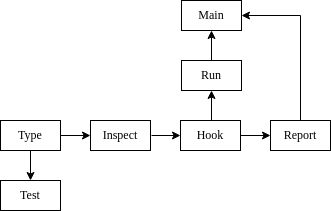
\includegraphics[width=0.45\textwidth]{pictures/module_diagram.png}
\caption{Diagram module}
\label{fig:diag}
\end{figure}






% Equation example 1:

% \begin{equation}
% \begin{split}
% \min_u \int_{x_i\in X}\int_{x_j\in X} q_{ij} u_i u_j da da + \int_{x_i\in X}||x' - x_i|| u_i da \\
% s.t. \ \ \ u\in[0,1] \ \ \land  \ \ \int_{x_i\in X}u da = a_0,
% \end{split}
% \end{equation}

% Equation exmaple 2:

% \begin{equation}
% \begin{split}
% \min_{\mathbf{u}} \alpha \mathbf{u}^T \mathbf{A}^T \mathbf{Q} \mathbf{A} \mathbf{u} +  \beta \mathbf{d}^T a' \mathbf{A} \mathbf{u} + \gamma \mathbf{u}^T \mathbf{G}^T \mathbf{G} \mathbf{u} + \delta\mathbf{f}^T a' \mathbf{A} \mathbf{u} \\
% s.t. \ \ \ \mathbf{0} \leq \mathbf{u} \leq \mathbf{1} \land \mathbf{a}^T\mathbf{u}=a_0.
% \end{split}
% \end{equation}

% Equation example 3:
% \begin{align}
% \mathbf{G}=(g_{ij}) = \left\lbrace
% \begin{array}{ll}
% \sum_{f_k\in N_f(f_i)} l_{ik} & i=j\\
% -l_{ij} & e_{ij}\in E\\
% 0 & \text{otherwise}
% \end{array}
% \right.
% \end{align}

% \lstinputlisting[label=mean,title={Mean Filter},caption={Mean Filter},language=R]{codes/mean.R}

% %% Poruguese algorithm
% %\begin{algorithm}
% %\DontPrintSemicolon
% %\Entrada{Malha e quantidade de pontos a ser amostrado}
% %\Saida{Pontos amostrados na malha}
% %\BlankLine
% %\emph{Crie um vetor de números randômicos entre $[0,1]$ com a %quantidade de pontos a ser amostrada e ordene-o}\;
% %\emph{Calcule a área total dos triângulos da malha}\;
% %\For{$i=0$ \KwTo numeroDePontos} {
% %  \emph{Navegue entre as faces acumulando a sua $\frac{area}{areaTotal}$ até achar a face com valor acumulado $\geqslant$ numerosRandomicos[i]}\;
% %  \emph{Pegue um ponto randômico dentro da face utilizando o %método de Turk e adicione no vetor do resultado}\;
% %}
% %\caption{Escolha das amostras inicias}\label{alg:sampling}
% %\end{algorithm}\DecMargin{1em}

% %% enlgish algorithm
% \begin{algorithm}
% \DontPrintSemicolon
% \KwIn{Malha e quantidade de pontos a ser amostrado}
% \KwOut{Pontos amostrados na malha}
% \BlankLine
% \emph{Crie um vetor de números randômicos entre $[0,1]$ com a quantidade de pontos a ser amostrada e ordene-o}\;
% \emph{Calcule a área total dos triângulos da malha}\;
% \For{$i=0$ \KwTo numeroDePontos} {
%   \emph{Navegue entre as faces acumulando a sua $\frac{area}{areaTotal}$ até achar a face com valor acumulado $\geqslant$ numerosRandomicos[i]}\;
%   \emph{Pegue um ponto randômico dentro da face utilizando o método de Turk e adicione no vetor do resultado}\;
% }
% \caption{Escolha das amostras inicias}\label{alg:sampling}
% \end{algorithm}\DecMargin{1em}




% \begin{flalign*}
%     && \left \{ l : \tau_i \right \} \cup \left \{ k : \tau_j \right \} = 
%     \left\{\begin{matrix}
%      \left \{ l_i : \tau_i \cup \tau_j \right \} &  \text{if} \ l = k\\ 
%      \left \{ l : \tau_i \cup nil, k:\tau_j \cup nil \right \} &  \text{if} \ l \neq  k\\ 
%     \end{matrix}\right. && \text{record union}
% \end{flalign*}
% \begin{flalign*}
%     \tau_i^{i\in 1..n} \cup  \tau_j^{j\in 1..m} = \left\{\begin{matrix}
%         \tau_i \cup \tau_j & \text{if} \ i = j\\ 
%         \tau_i \cup nil & \text{if} \ i > m\ \\
%         \tau_j \cup nil & \text{if} \ j > n\ \\
%        \end{matrix}\right. && \text{function union}
% \end{flalign*}
% \begin{flalign*}
%     \tau \cup nil = \tau? && \text{nil union}
% \end{flalign*}


%  \begin{center}
%     \( \left \{ \left. \tau_i \right \}\right. \cup \left \{ \left. \tau_j \right \}\right. = \left \{ \left. \tau_i \cup \tau_j \right \}\right. \)
% \end{center}

% \begin{center}
%     \( \left \{ l : \tau_i \right \} \cup \left \{ k : \tau_j \right \} = 
%     \left\{\begin{matrix}
%      \left \{ l_i : \tau_i \cup \tau_j \right \} &  \text{if} \ l = k\\ 
%      \left \{ l : \tau_i \cup nil, k:\tau_j \cup nil \right \} &  \text{if} \ l \neq  k\\ 
%     \end{matrix}\right. \)
% \end{center}

% \begin{center}
%     \(  \tau_i^{i\in 1..n} \cup  \tau_j^{j\in 1..m} = \left\{\begin{matrix}
%         \tau_i \cup \tau_j & \text{if} \ i = j\\ 
%         \tau_i \cup nil & \text{if} \ i > m\ \\
%         \tau_j \cup nil & \text{if} \ j > n\ \\
%        \end{matrix}\right. \)
% \end{center}
% \par
% First, the primitive types are some of the Lua basic types, added by the distinction between \textit{integer} and \textit{float}. It does not add any complexity for the types already defined by the language. The syntax of an array type is denoted by a pair of brackets with a single type. A record type is denoted by a pair of brackets with a list of labels and their respective types The \(l : \tau\) representation means that the label \textit{l} has type \(\tau\). Similarly, a function type is represented by two lists of types, where the left part represents the parameter types, while the other one represents the return types. Finally, an optional type is denoted by a type followed by a question mark.

% First, the primitive types are some of the Lua basic types, added by the distinction between \textit{integer} and \textit{float}. It does not add any complexity for the types already defined by the language:
% \begin{center}
%     \(primitive \ types\ :=\ nil \;|\; boolean \;|\; integer \;|\; float \;|\; number \;|\; string\)
% \end{center}
% The syntax of an array type is denoted by a pair of brackets with a single type:
% \begin{center}
%     \(array \ type\ :=\ \left \{ \tau \right \}\)
% \end{center}
% A record type is denoted by a pair of brackets with a list of labels and their respective types The \(l : \tau\) representation means that the label \textit{l} has type \(\tau\).
% \begin{center}
%     \(record \ type\ :=\ \left \{ l_i : \tau_i \right \} ^ {i \in 1..n} \)
% \end{center}
% Similarly, a function type is represented by two lists of types, where the left part represents the parameter types, while the other one represents the return types
% \begin{center}
%     \(function \ type\ :=\ \tau_i ^ {i \in 1..n} \rightarrow \tau_j ^ {j \in 1..m} \)
% \end{center}
% Finally, an optional type is denoted by a type followed by a question mark.
% \begin{center}
%     \(optional \ type\ :=\ \tau?\)
% \end{center}

% \begin{flalign*}
%     && \tau&:=nil \;|\; boolean \;|\; integer \;|\; float \;|\; number \;|\; string && \text{primitive types} \\
%     && &| \ \left \{ \tau \right \} && \text{array type} \\
%     && &| \ \left \{ l_i : \tau_i \right \} ^ {i \in 1..n} && \text{record type} \\
%     && &| \ \tau_i ^ {i \in 1..n} \rightarrow \tau_j ^ {j \in 1..m}  && \text{function type}
%     \end{flalign*}

% \begin{align*}
%     \tau&:=nil \;|\; boolean \;|\; integer \;|\; float \;|\; number \;|\; string \\ 
%     &| \ \left \{ \tau \right \} \\ 
%     &| \ \left \{ l_i : \tau_i \right \} ^ {i \in 1..n} \\ 
%     &| \ \tau_i ^ {i \in 1..n} \rightarrow \tau_j ^ {j \in 1..m} 
%    \end{align*}
%    \begin{align*}
%     &\qquad \textit{primitive types} \\ 
%     &\qquad  \textit{array type} \\
%     &\qquad  \textit{record type} \\
%     &\qquad  \textit{function type}
%    \end{align*}
   

%  \begin{center}
%   \begin{tabular}{l}
%     \(primitive \ types\ :=\ nil \;|\; boolean \;|\; integer \;|\; float \;|\; number \;|\; string\) \\
%     \(array \ type\ :=\ \left \{ \tau \right \}\) \\
%     \(record \ type\ :=\ \left \{ l_i : \tau_i \right \} ^ {i \in 1..n} \) \\
%     \(function \ type\ :=\ \tau_i ^ {i \in 1..n} \rightarrow \tau_j ^ {j \in 1..m} \) \\
%     \(optional \ type\ :=\ \tau?\)
%   \end{tabular}
%  \end{center}
%  Primitive types are some of Lua basic types, added by the distinction between \textit{integer} and \textit{float}. The array, record and function types are recursive definitions, it means that the symbol \(\tau\) can represent any of the type definitions. The syntax of an array type is denoted by a pair of brackets with a single type. A record type is denoted by a pair of brackets with a list of labels and their respective types The \(l : \tau\) representation means that the label \textit{l} has type \(\tau\). Similarly, a function type is represented by two lists of types, where the left part represents the parameter types, while the other one represents the return types. At last, an optional type is denoted by the type definition followed by a question mark.
 
% \begin{flalign*}
%     && \left \{ \left. \tau_i \right \}\right. \cup \left \{ \left. \tau_j \right \}\right. = \left \{ \left. \tau_i \cup \tau_j \right \}\right. && \text{array union} \\ \\
%     && \left \{ l : \tau_i \right \} \cup \left \{ k : \tau_j \right \} = 
%     \left\{\begin{matrix}
%      \left \{ l_i : \tau_i \cup \tau_j \right \} &  \text{if} \ l = k\\ 
%      \left \{ l : \tau_i \cup nil, k:\tau_j \cup nil \right \} &  \text{if} \ l \neq  k\\ 
%     \end{matrix}\right. && \text{record union} \\ \\
%     && \tau_i^{i\in 1..n} \cup  \tau_j^{j\in 1..m} = \left\{\begin{matrix}
%         \tau_i \cup \tau_j & \text{if} \ i = j\\ 
%         \tau_i \cup nil & \text{if} \ i > m\ \\
%         \tau_j \cup nil & \text{if} \ j > n\ \\
%        \end{matrix}\right. && \text{funciton union} \\ \\
%     && \tau \cup nil = \tau? && \text{nil union} \\ \\ 
%     && integer \cup float = number && \text{nil union}
% \end{flalign*}


